\documentclass[12pt, titlepage]{article}

\usepackage{booktabs}
\usepackage{tabularx}
\usepackage{hyperref}
\usepackage{graphicx}
\usepackage{enumitem}
\hypersetup{
	colorlinks,
	citecolor=black,
	filecolor=black,
	linkcolor=red,
	urlcolor=blue
}
\usepackage[numbers]{natbib}

\title{SE 3XA3: Software Requirements Specification\\Wordle 2.0}

\author{Team 8, Goufs
	\\ Richard Fan, fanr13
	\\ Noel Zacharia, zacharin
	\\ Biranugan Pirabaharan, pirabahb
}

\date{\today}

\begin{document}
	
	\maketitle
	
	\pagenumbering{roman}
	\tableofcontents
	\listoftables
	\listoffigures
	
	\begin{table}[bp]
		\caption{\bf Revision History}
		\begin{tabularx}{\textwidth}{p{3cm}p{2cm}X}
			\toprule {\bf Date} & {\bf Version} & {\bf Notes}\\
			\midrule
			Feb 7, 2022  & 1.0 & Initial Document\\
			Feb 9, 2022 & 1.1 & More sections added\\
			Feb 10, 2022 & 1.2 & Use case diagram and final sections added\\
			Feb 10, 2022 & 1.3 & Final revision and check \\
			\bottomrule
		\end{tabularx}
	\end{table}
	
	\newpage
	
	\pagenumbering{arabic}
	This document describes the requirements for the game Wordle 2.0. The 
	template 
	for this Software Requirements Specification is a subset of the Volere 
	template[1].
	
	
	\section{Project Drivers}
	
	\subsection{The Purpose of the Project}
	The purpose of this project is to recreate the functionality of the web 
	game Wordle. Additionally, we aim to modernize the UI and add new features 
	such as a dark mode and more levels.
	\subsection{The Stakeholders}
	
	\subsubsection{The Client}
	The client is the professor for this course, Dr. Asghar Bokahri, and the 
	teaching assistants, Veerash Palanichamy, Oluwaseun Owojaiye, and Abdul Rab 
	Mohammed. The clients will provide us with deadlines on deliverables, and 
	will 
	have the final decision on the project's acceptance and adherence to the 
	SRS. 
	
	\subsubsection{The Customers}
	In this case, the customers are all people who will play the Wordle 2.0 
	game. 
	This game targets people of a demographics and will have minimal hardware 
	requirements to decrease the barriers to access.
	
	\subsubsection{Other Stakeholders}
	The developers of this project are also stakeholders. Without them, there 
	would 
	be no Wordle 2.0. The skills of individual team members, both technical and 
	soft skills, will be put to use to complete this project. They 
	will be 
	responsible for the implementation, documentation, and testing of the 
	product. 
	Additionally, the original developers and contributors to the Wordle Clone 
	repository will be stakeholders in this project as they are constantly 
	updating the respository and wish to improve the game.
	
	\subsection{Mandated Constraints}
	\subsubsection{Solution Constraints}
	\noindent \textbf{Description:} Wordle must be able to run on any modern 
	browser or laptop.\\
	\textbf{Rationale:} The potential users of Wordle will need to have the 
	listed browsers. \\
	\textbf{Fit Criterion:} Wordle will run on any latest version of node.
	
	\subsubsection{Implementation Environment of the Current System}
	\noindent \emph{N/A}
	
	\subsubsection{Partner or Collaborative Applications}
	\noindent \emph{N/A}
	
	\subsubsection{Off-the-Shelf Software}
	\noindent \emph{N/A}
	
	\subsubsection{Anticipated Workplace Environment}
	\noindent \emph{N/A}
	
	\subsubsection{Schedule Constraints}
	\noindent \textbf{Description:} The Project must follow the project 
	schedule shown in the Development Plan\\
	\textbf{Rationale:} The Project needs to follow a predefined plan 
	to ensure the completion of the milestones by their respective due dates. \\
	\textbf{Fit Criterion:} The Project will be completed with all milestones 
	submitted on time. 
	
	\subsubsection{Budget Constraints}
	\noindent \emph{N/A}
	
	\newpage
	\subsection{Naming Conventions and Terminology}
	\begin{table}[h!]
		\caption{Naming Conventions and Terminology}
		\begin{tabular}{ |p{6cm}|p{8cm}|  }
			\hline
			\multicolumn{2}{|c|}{Naming Conventions and Terminology} \\
			\hline
			\textbf{Term} & \textbf{Definition}\\
			\hline
			JavaScript(JS) & The programming language used in this project.  \\
			\hline
			Player/User & The individual playing the game.   \\
			\hline
			TypeScript & The programming language used in Not Wordle.  \\
			\hline
			System    & The software behind the game.  \\
			\hline 
			SRS & Acronym meaning Software Requirments Specification. This 
			document 
			describes what the software system is to do and its expected 
			performance.   \\
			\hline
			Web Browser & The platform on which the game will run. \\
			\hline
			User Interface & The point at which the user interacts with the 
			system.  \\
			\hline
			React & The JS library that is used for building the user 
			interface.  \\
			\hline
		\end{tabular}
	\end{table}
	
	\subsection{Relevant Facts and Assumptions}
	
	Facts:\\ The original repository is still being updated constantly. 
	However, 
	we
	are implementing and improving the version of the repository we found at the
	start of the term. This is to avoid having the original repository grow too
	large for the scope of our project. \\ Originally the repository did not 
	have
	a dark theme, various word length game modes, or hard mode where all guesses
	must contain correct letters from previous guesses. \\ Assumptions: \\ 
	Users will use a system with a web
	browser and have internet access. \\ Users will know how to operate a
	computer or phone.\\ Users have a moderate proficiency in English, at least 
	a
	middle school level.
	
	\section{Functional Requirements}
	
	\subsection{The Scope of the Work and the Product}
	
	\subsubsection{The Context of the Work}
	Wordle 2.0 is a standalone application that doesn't interact with other 
	folders or systems. It is meant to be played by one person at a time.
	\newpage
	\subsubsection{Work Partitioning}
	
	\begin{table}[h!]
		\caption{Work Partitioning Events}
		\centering
		\begin{tabular}{|c|p{3.5cm}|c|p{3.5cm}|}
			\hline
			\textbf{Event Number} & \centering\textbf{Event Name} & 
			\textbf{Input} 
			& \textbf{Output} \\
			\hline
			1 & Starting a new game & Mouse & Final Score \\
			\hline
			2 & Reading the instructions  & Mouse & Instructions shown \\
			\hline
			3 & Opening the settings menu & Mouse & Settings shown \\
			\hline
			4 & Viewing about & Mouse & About \\
			\hline
		\end{tabular}
	\end{table}
	\begin{table}[h]
		\caption{Work Partitioning Summaries}
		\centering
		\begin{tabular}{|c|p{11cm}|}
			\hline
			\textbf{Event Number} & \textbf{Summary} \\
			\hline
			1 & The user will use the mouse to start a 
			new game. When the game ends, the user will see the hidden word 
			and a summary of their guesses. \\
			\hline
			2 & The user using the mouse, decides to read the instructions of 
			Wordle 2.0. \\
			\hline
			3 & During the game, the user can use the mouse to open the 
			settings 
			menu. \\
			\hline
			4 &  The user, through mouse input, views the about page.\\
			\hline
		\end{tabular}
	\end{table}
	\newpage
	
	\subsubsection{Individual Product Use Cases}
	\begin{figure}[h]
		\centering
		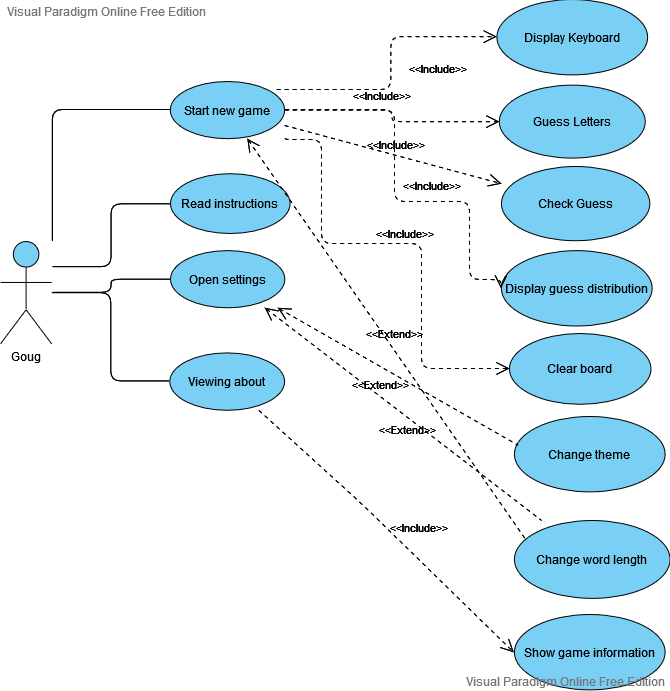
\includegraphics[width=12cm, height=13cm]{usecase.png}
		\caption{Use case diagram that displays the main functionalities of the 
			application.}
	\end{figure}
	
	
	\newpage
	\subsection{Functional Requirements} FR1. The system must display the 
	letters
	in a keyboard layout, along with the enter and delete options. \\ FR2. The
	system must display the 6 rows for attempts, each having 5 boxes for the
	letters. \\ FR3. The system must have an option to change the theme of the
	page. \\ FR4. The system must have an option to display the rules of the 
	game. \\
	FR5. The system must have an option to display the player’s statistics. \\ 
	FR6.
	The system must display the player’s total games played. \\ FR7. The system
	must display the success rate of the player. \\ FR8. The system must display
	the current streak of correct guesses made. \\ FR9. The system must display 
	the
	player’s best streak of correct guesses. \\ FR10. The system must display 
	the
	player’s guess distribution (distribution of the number of attempts a
	correct guess took). \\ FR11. The system must have a share option (copies 
	the
	result of their last game to their clipboard as emojis) \\ FR12. The system
	must allow the user to make a guess \\ FR13. The system must display if a
	letter is in the correct position in the target word. \\ FR14. The system 
	must
	display if a letter is in the target word but not in the correct position.
	\\ FR15. The system must display if a letter is not in the target word. \\ 
	FR16.
	The system must alert the player if their guess is not a valid word. \\ 
	FR17.
	The system must alert the player if their guess does not contain enough
	letters. \\ FR18. The system must update the displayed keyboard to reflect 
	the
	accuracy of the letters guessed. \\ FR19. The system must prohibit the user 
	from
	changing their guess after they submit it. \\ FR20. The system must have an
	option to the game mode (word length to either 4 or 6). \\ FR21. The system
	must update the display to reflect the game mode. \\ FR22. The system must 
	give an
	option to play again, giving the player a new target word and resetting the
	display to its initial state. 
	\newpage
	\section{Non-functional Requirements}
	
	\subsection{Look and Feel Requirements}
	\subsubsection{Appearance Requirements}
	LF1 The UI must be easy to understand and use.
	\subsubsection{Style Requirements}
	LF2 The UI theme must be inspired by wordle's UI.
	
	\subsection{Usability and Humanity Requirements}
	\begin{enumerate}[label=UH\arabic*]
		\item The game must be understood by users between the ages of 
		$\hyperlink{min_age}{MIN\_AGE}$ and $\hyperlink{min_age}{MAX\_AGE}$.
		\item The game must be playable with the use of only one hand.
		\item The game must provide themes to best suit the user's environment.
		\item The game must be playable with no background knowledge.
		\item The game must have two methods of input(keyboard/mouse) to best 
		suit 
		the user's preferences.
	\end{enumerate}
	
	\subsection{Performance Requirements}
	\begin{enumerate}[label=P\arabic*]
		\item The system must update the display quickly (within 
		$\hypertarget{min_time}{MIN\_TIME}$ seconds) 
		whenever the user has input.
		\item The system must load all visuals on startup within 
		$\hypertarget{min_time}{MIN\_TIME}$ seconds. 
		\item The system must update the statistics within 
		$\hypertarget{min_time}{MIN\_TIME}$ seconds after the 
		last 
		game has ended. 
	\end{enumerate}
	
	\subsection{Operational and Environmental Requirements}
	\subsubsection{Expected Physical Environment}
	OR1 The system must not require an internet connection nor should it 
	require 
	high-performance graphic cards.
	\subsubsection{Requirements for Interfacing with Adjacent Systems}
	OR2 The program should not access and make changes to any file outside its 
	own 
	folder
	\subsubsection{Productization Requirements}
	OR3 The game must be distributed as a zip folder and its total size must be 
	below $\hypertarget{max_storage}{MAX\_STORAGE}$.
	\subsubsection{Release Requirements}
	OR4 The product will have a final release date corresponding to the last 
	day 
	of 
	classes.
	\subsection{Maintainability and Support Requirements}
	\begin{enumerate}[label=M\arabic*]
		\item The code must be documented through the use of comments and 
		\item The code must follow the style agreed upon in the Development 
		Plan.
		\item Any changes will be documented.  
	\end{enumerate}
	
	\subsection{Security Requirements}
	
	SR1. The user must not be able to view the statistics of other players.
	
	\subsection{Cultural Requirements}
	\subsubsection{Cultural Requirements}
	CR1 The game can't suggest offensive words or non-English words.
	
	\subsubsection{Political Requirements}
	CR 2 The game can't suggest politically charged words.
	
	\subsection{Legal Requirements}
	\begin{enumerate}[label=LR\arabic*]
		\item The program must not break any digital privacy laws within the 
		countries of 
		Canada 
		and the United States of America.
	\end{enumerate}
	\subsection{Health and Safety Requirements}
	\begin{enumerate}[label=HS\arabic*]
		\item The project will not include any form of high-frequency flashes, 
		contrast 
		alteration, or brightness variation which may cause epileptic seizures 
		for 
		some 
		users.
		\item To prevent repetitive stress injury and addiction, a warning will 
		be 
		displayed by the system encouraging users to take regular breaks.
	\end{enumerate}
	\section{Project Issues}
	
	\subsection{Open Issues} We have not decided on a testing framework as no
	Javascript framework is considered the best solution according to the
	programming community. Currently leaning towards using JEST or Cypress, but
	still exploring the limitations of each. \\
	We are also not proficient with TypeScript, thus it is uncertain how 
	difficult it will be to modularize the source code as it is written in 
	TypeScript. 
	
	\subsection{Off-the-Shelf Solutions}
	Wordle is the original version of this game. However, its source code is 
	not 
	published. There are few public solutions specific to the creation of 
	Wordle 
	2.0; any code adapted for the project will come from Not Wordle.
	\subsubsection{Ready-Made Products}
	Wordle Clones exist in the market. One such example is the source 
	repository.
	\subsubsection{Reusable Components}
	The source repository has resusable components that can be replicated on a 
	need-to-need basis.
	\subsubsection{Products That Can Be Copied}
	The source repository has an MIT licence and thus redistribution or 
	replication 
	of the product is allowed.
	
	\subsection{New Problems}
	
	\subsection{Tasks} Tasks are assigned and specified using a \href
	{https://gitlab.cas.mcmaster.ca/zacharin/wordle_clone_3xa3_l01_group8/-/blob/main/ProjectSchedule/3xa3_group8.gan}{\color{blue}Gantt
		Chart}. The chart is maintained and updated through the lifetime of the
	product’s development. 
	
	\subsection{Migration to the New Product}
	N/A. This product will remain independent of the source code.
	\subsection{Risks}
	There is little to no risk associated with this project. 
	The 
	program is designed to run within a web browser which has very little 
	interaction with other processes running within the user's system. Any 
	risks stemming from the program itself may occur in the form of crashes and 
	ppoor performance. Test driven development will be done to minimize these 
	risks.
	\subsection{Costs}
	
	The development of the project will have no cost. Under the MIT licence, the
	source project is allowed to be modified and distributed freely. 
	The
	applications used for development are also free. An estimated time cost for
	development is 6 hours a week for all developers. 
	
	\subsection{User Documentation and Training}
	\subsubsection{User Documentation Requirements}
	Instructions will be included as an option in the game's main menu.
	The game's directory will contain a README file providing installation 
	instructions.
	
	\subsubsection{Training Requirements}
	No specific training is necessary to play Wordle 2.0. Controls should be 
	intuitive.
	
	\subsection{Waiting Room}
	Should there be additional time, the following low priority features will 
	be 
	considered and implemented:
	
	\begin{enumerate}
		\item Different world lengths. The user would be able to change the 
		gameplay mode to include words that are not 5 letters in length
		\item Allow for multiplayer functionality.
	\end{enumerate}
	
	\subsection{Ideas for Solutions}
	N/A.
	
	\bibliography{cite}
	\bibliographystyle{ieeetr}
	\nocite{*}
	
	\newpage
	
	\section{Appendix}
	
	\subsection{Symbolic Parameters}
	$\hypertarget{min_age}{MIN\_AGE}$ = 10\\
	$\hypertarget{min_age}{MAX\_AGE}$ = 90\\
	$\hypertarget{max_storage}{MAX\_STORAGE}$ = 20\\
	$\hypertarget{min_time}{MIN\_TIME}$ = 0.25\\
	
	
\end{document}